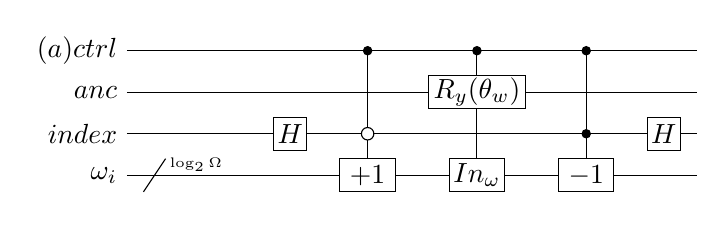
\begin{tikzpicture}[scale=1.000000,x=1pt,y=1pt]
\filldraw[color=white] (0.000000, -7.500000) rectangle (206.000000, 52.500000);
% Drawing wires
% Line 1: ctrl W \text{(a) }ctrl
\draw[color=black] (0.000000,45.000000) -- (206.000000,45.000000);
\draw[color=black] (0.000000,45.000000) node[left] {$\text{(a) }ctrl$};
% Line 2: anc W anc
\draw[color=black] (0.000000,30.000000) -- (206.000000,30.000000);
\draw[color=black] (0.000000,30.000000) node[left] {$anc$};
% Line 3: index W index
\draw[color=black] (0.000000,15.000000) -- (206.000000,15.000000);
\draw[color=black] (0.000000,15.000000) node[left] {$index$};
% Line 4: i W \omega_i
\draw[color=black] (0.000000,0.000000) -- (206.000000,0.000000);
\draw[color=black] (0.000000,0.000000) node[left] {$\omega_i$};
% Done with wires; drawing gates
% Line 6: i / ^{\log_2{\Omega}}
\draw (6.000000, -6.000000) -- (14.000000, 6.000000);
\draw (12.000000, 3.000000) node[right] {$\scriptstyle{^{\log_2{\Omega}}}$};
% Line 7: ctrl anc index i LABEL
% Line 9: index G $H$
\begin{scope}
\draw[fill=white] (59.000000, 15.000000) +(-45.000000:8.485281pt and 8.485281pt) -- +(45.000000:8.485281pt and 8.485281pt) -- +(135.000000:8.485281pt and 8.485281pt) -- +(225.000000:8.485281pt and 8.485281pt) -- cycle;
\clip (59.000000, 15.000000) +(-45.000000:8.485281pt and 8.485281pt) -- +(45.000000:8.485281pt and 8.485281pt) -- +(135.000000:8.485281pt and 8.485281pt) -- +(225.000000:8.485281pt and 8.485281pt) -- cycle;
\draw (59.000000, 15.000000) node {$H$};
\end{scope}
% Line 10: i G width=20 $+1$ ctrl -index
\draw (87.000000,45.000000) -- (87.000000,0.000000);
\begin{scope}
\draw[fill=white] (87.000000, -0.000000) +(-45.000000:14.142136pt and 8.485281pt) -- +(45.000000:14.142136pt and 8.485281pt) -- +(135.000000:14.142136pt and 8.485281pt) -- +(225.000000:14.142136pt and 8.485281pt) -- cycle;
\clip (87.000000, -0.000000) +(-45.000000:14.142136pt and 8.485281pt) -- +(45.000000:14.142136pt and 8.485281pt) -- +(135.000000:14.142136pt and 8.485281pt) -- +(225.000000:14.142136pt and 8.485281pt) -- cycle;
\draw (87.000000, -0.000000) node {$+1$};
\end{scope}
\filldraw (87.000000, 45.000000) circle(1.500000pt);
\draw[fill=white] (87.000000, 15.000000) circle(2.250000pt);
% Line 11: anc G:width=35 $R_y(\theta_w)$ i G:width=20 $In_\omega$ ctrl
\draw (126.500000,45.000000) -- (126.500000,0.000000);
\begin{scope}
\draw[fill=white] (126.500000, 30.000000) +(-45.000000:24.748737pt and 8.485281pt) -- +(45.000000:24.748737pt and 8.485281pt) -- +(135.000000:24.748737pt and 8.485281pt) -- +(225.000000:24.748737pt and 8.485281pt) -- cycle;
\clip (126.500000, 30.000000) +(-45.000000:24.748737pt and 8.485281pt) -- +(45.000000:24.748737pt and 8.485281pt) -- +(135.000000:24.748737pt and 8.485281pt) -- +(225.000000:24.748737pt and 8.485281pt) -- cycle;
\draw (126.500000, 30.000000) node {$R_y(\theta_w)$};
\end{scope}
\begin{scope}
\draw[fill=white] (126.500000, -0.000000) +(-45.000000:14.142136pt and 8.485281pt) -- +(45.000000:14.142136pt and 8.485281pt) -- +(135.000000:14.142136pt and 8.485281pt) -- +(225.000000:14.142136pt and 8.485281pt) -- cycle;
\clip (126.500000, -0.000000) +(-45.000000:14.142136pt and 8.485281pt) -- +(45.000000:14.142136pt and 8.485281pt) -- +(135.000000:14.142136pt and 8.485281pt) -- +(225.000000:14.142136pt and 8.485281pt) -- cycle;
\draw (126.500000, -0.000000) node {$In_\omega$};
\end{scope}
\filldraw (126.500000, 45.000000) circle(1.500000pt);
% Line 12: i G width=20 $-1$ ctrl index
\draw (166.000000,45.000000) -- (166.000000,0.000000);
\begin{scope}
\draw[fill=white] (166.000000, -0.000000) +(-45.000000:14.142136pt and 8.485281pt) -- +(45.000000:14.142136pt and 8.485281pt) -- +(135.000000:14.142136pt and 8.485281pt) -- +(225.000000:14.142136pt and 8.485281pt) -- cycle;
\clip (166.000000, -0.000000) +(-45.000000:14.142136pt and 8.485281pt) -- +(45.000000:14.142136pt and 8.485281pt) -- +(135.000000:14.142136pt and 8.485281pt) -- +(225.000000:14.142136pt and 8.485281pt) -- cycle;
\draw (166.000000, -0.000000) node {$-1$};
\end{scope}
\filldraw (166.000000, 45.000000) circle(1.500000pt);
\filldraw (166.000000, 15.000000) circle(1.500000pt);
% Line 13: index G $H$
\begin{scope}
\draw[fill=white] (194.000000, 15.000000) +(-45.000000:8.485281pt and 8.485281pt) -- +(45.000000:8.485281pt and 8.485281pt) -- +(135.000000:8.485281pt and 8.485281pt) -- +(225.000000:8.485281pt and 8.485281pt) -- cycle;
\clip (194.000000, 15.000000) +(-45.000000:8.485281pt and 8.485281pt) -- +(45.000000:8.485281pt and 8.485281pt) -- +(135.000000:8.485281pt and 8.485281pt) -- +(225.000000:8.485281pt and 8.485281pt) -- cycle;
\draw (194.000000, 15.000000) node {$H$};
\end{scope}
% Done with gates; drawing ending labels
% Done with ending labels; drawing cut lines and comments
% Done with comments
\end{tikzpicture}
